%%%%%%%%%%%%%%%%%%%%%%%%%%%%%%%%%%%%%%%%%
% Kieker Analysis Component
% 
% $Date$
% $Rev$:
% $Author$


\chapter{\KiekerAnalysisPart{} Component}\label{chap:componentsAnalysis}

\NOTIFYBOX{The Java sources of this chapter can also be found in the %
\file{\customComponentsBookstoreApplicationDirDistro{}/} directory of the %
binary release.}

\section{Analysis Controller}\label{sec:analysis:controller}

An analysis with \KiekerAnalysisPart{} is set up and executed employing %
the class \class{AnalysisController}. %
\KiekerAnalysisPart{} requires a monitoring reader %
(Section~\ref{sec:analysis:reader}) and at least %
one monitoring record consumer plugin (Section~\ref{sec:analysis:consumer}). %
In addition to the monitoring record consumer plugin, %
other analysis plugins can be registered. %
Figure~\ref{fig:analysisController:classdiagram} shows the class diagram %
with the important \KiekerAnalysisPart{} classes and their relationship. %

\begin{figure}[h]\centering
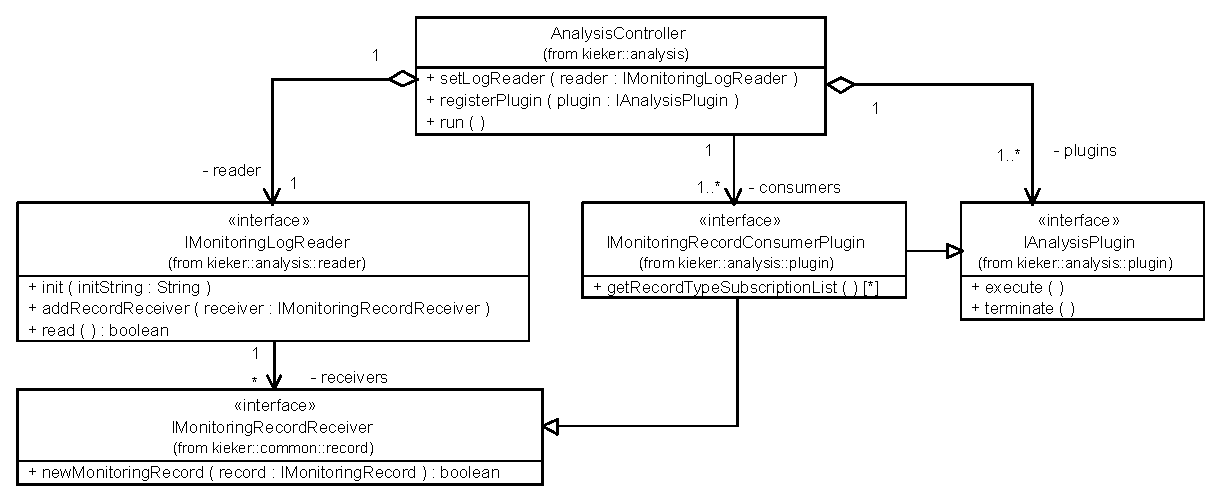
\includegraphics[scale=0.65]{images/kieker_AnalysisControlleruserguide-modified}
\caption{Class diagram showing important \KiekerAnalysisPart{} classes and their relationship}
\label{fig:analysisController:classdiagram}
\end{figure}

\noindent Setting up and running an analysis with \KiekerAnalysisPart{} requires the %
following steps to be performed, as described in Section~\ref{sec:example:analysis} already:\\

\enlargethispage{1cm}

\begin{compactenum}
\item Creating an instance of the \class{AnalysisController} class
\item Creating and registering the monitoring reader (\method{setReader}) as %
well as the monitoring record consumers and other analysis plugins (\method{registerPlugin}).
\item Starting the analysis instance (\method{run}).
\end{compactenum}

\

\noindent In the following Sections~\ref{sec:analysis:reader} and~\ref{sec:analysis:consumer}, %
we will create a custom monitoring reader \class{MyPipeReader} and a %
monitoring record consumer plugin \class{MyResponseTimeConsumer}. %
\noindent The following Listing~\ref{listing:AnalysisController} shows how to create and run an analysis %
with these custom components:

\setJavaCodeListing
\lstinputlisting[caption=Code snippet setting up and running a \KiekerAnalysisPart{} instance (Starter.java),label=listing:AnalysisController,firstline=46, lastline=53, firstnumber=46]%
{\customComponentsBookstoreApplicationDir/src/bookstoreApplication/Starter.java}

\enlargethispage{1.2cm}

\noindent On invocation of the \method{run} method, the \class{Analysis Controller} %
calls the \method{execute} method of all analysis plugins allowing them to initialize. %
Then, it starts the configured monitoring reader by calling its \method{read} %
method. Monitoring record consumers receive the monitoring records provided by %
the reader. As soon as the reader returns from the execution of its \method{read} 
method, the method \method{terminate} of each registered plugin is called by the %
\class{Analysis Controller}. %
In order to support the asynchronous execution of the \class{AnalysisController} instance, %
we provide the \class{AnalysisControllerThread} class.

\section{Monitoring Readers}\label{sec:analysis:reader}

% Warning-tag for the reader-writer-thing
The monitoring readers are the direct counterpart to the monitoring %
writers. While writers receive records and write them into files or other kinds %
of monitoring logs/streams, readers deserialize monitoring data and provide it as %
\class{IMonitoringRecord} instances. 

\begin{figure}[h]\centering
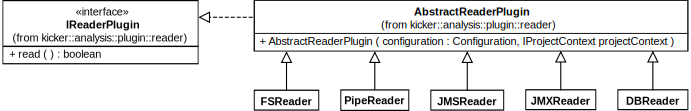
\includegraphics[scale=0.7]{images/kieker_readerimplsuserguide-modified}
\caption{Interface \class{IMonitoringReader} and implementing classes}
\label{Figure:ReaderHierarchy}
\end{figure}

\pagebreak

% \
% 
% \WARNBOX{This means that whenever a new writer is implemented, a corresponding reader has to be implemented as well. If one want for example to store the recorded informations in a database, one should be capable of reading these saved informations from the database again.}
% 
% \

% \enlargethispage{1cm}

\noindent There are already some readers implemented in \Kieker,  as shown in the %
class diagram in Figure \ref{Figure:ReaderHierarchy}. %
The \class{FSReader} has already been used in Section~\ref{sec:example:analysis}. %
The \class{FSReaderRealtime} can be used to simulate continuous monitoring of a %
production system. It adds delays between the delivery of the monitoring records %
to its consumers according to the original delays reconstructed from the logging %
timestamps (Section~\ref{sec:componentsMonitoring:monitoringRecords}).
A brief description of how to use the \class{JMSReader} can be found in Appendix~\ref{appendix:usingJMS}. %

\noindent The implementation of a custom reader is similar to the implementation of a %
monitoring writer. Custom readers should extend the class \class{AbstractKiekerMonitoringReader} %
which already provides an implementation of the observer pattern. %
By invoking the method \method{deliverRecord},  the delivery of records is then %
delegated to the super class.

Listing~\ref{listing:MyReader} on page~\pageref{listing:MyReader} shows a simple reader which polls records from %
the named pipe introduced in the previous Chapter~\ref{chap:componentsMonitoring}. %

% If there is nothing on the pipe to be read, the reader waits 4 seconds at maximum before it terminates.

\setJavaCodeListing
\lstinputlisting[firstline=29, firstnumber=29, caption=MyPipeReader.java (excerpt), label=listing:MyReader,float]{\customComponentsBookstoreApplicationDir/src/bookstoreApplication/MyPipeReader.java}

\section{Analysis Plugins}\label{sec:analysis:plugins}

Any analysis or visualization component used with \KiekerAnalysisPart{} must %
implement the interface \class{IAnalysisPlugin} (Figure~\ref{fig:analysisController:classdiagram}). %
As described in Section~\ref{sec:analysis:controller}, the life-cycle of each %
registered plugin is controlled by the \class{Analysis Controller} instance %
employing the methods \method{execute} and \method{terminate}. Analysis plugins %
must implement these methods for initialization and termination.

The monitoring record consumer plugins described in the following %
Section~\ref{sec:analysis:consumer}, are special analysis plugins that receive %
the monitoring records provided by the monitoring reader. %
Starting with these monitoring record plugins, analysis plugins can be connected %
in a pipe-and-filter style to implement more complex analyses. %
\Kieker{} provides input and output port interfaces and implementing classes %
to implement such analyses. See the documentation of the classes \class{AbstractInputPort} %
and \class{OutputPort} for details. \KiekerTraceAnalysis{} is implemented %
based on this pattern. 

\section{Monitoring Record Consumer Plugins}\label{sec:analysis:consumer}

As just mentioned, consumer plugins are special analysis plugins which receive %
the records provided by the monitoring reader and implement analyses or %
visualizations based on these records. %
Consumer plugins must implement the interface \class{IMonitoringRecordConsumerPlugin} %
(see Figure~\ref{fig:analysisController:classdiagram}). %
By implementing the \method{getRecordTypeSubscriptionList} method, a consumer plugin %
can specify the desired types of monitoring records to be received via the %
method \method{newMonitoringRecord}.

The custom consumer in Listing~\ref{lst:MyReponseTimeConsumer} on %
page~\pageref{lst:MyReponseTimeConsumer} simply writes %
the content of the received response time records to the standard output stream.

\pagebreak

\setJavaCodeListing
\lstinputlisting[caption=MyReponseTimeConsumer.java,label=lst:MyReponseTimeConsumer,firstline=21,firstnumber=21]{\customComponentsBookstoreApplicationDir/src/bookstoreApplication/MyResponseTimeConsumer.java}
